\documentclass[10pt,twocolumn,letterpaper]{article}
\providecommand{\src}[1]{}
\providecommand{\val}[2][1]{}
\usepackage[review]{cvpr}
\makeatletter\@ifpackageloaded{natbib}{}{\usepackage[numbers,sort&compress]{natbib}}\makeatother
\usepackage{graphicx}
\usepackage{booktabs}
\usepackage{amsmath}
\usepackage{amssymb}
\usepackage{xcolor}
\makeatletter\@ifpackageloaded{hyperref}{}{\usepackage[hidelinks]{hyperref}}\makeatother
% Unicode engines (XeTeX, LuaTeX) have no OpenType shapes for the Type 1 families that cvpr.sty loads through
% the times package, so bold and italic are lost. Load the TeX Gyre equivalents there; pdfTeX needs nothing.
\usepackage{iftex}
\ifPDFTeX\else
  \usepackage[no-math]{fontspec}
  \defaultfontfeatures{Extension=.otf, UprightFont=*-regular, BoldFont=*-bold, ItalicFont=*-italic,
    BoldItalicFont=*-bolditalic, Ligatures=TeX}
  \setmainfont{texgyretermes}
  \setsansfont{texgyreheros}
  \setmonofont[Ligatures=ResetAll]{texgyrecursor}
  \defaultfontfeatures{}
\fi

\def\paperID{*****}
\def\confName{CVPR}
\def\confYear{2026}

\title{Drop What the Model Disagrees With: Out-of-Fold Filtering for Label Noise}
\author{Anonymous Authors \\ Anonymous Institution}

\begin{document}
% Fig. 1 spans both columns under the title. Inside this box \maketitle must not open a second \twocolumn.
\twocolumn[{%
  \renewcommand\twocolumn[1][]{#1}%
  \maketitle
  % Fig. 1, set across both columns in the title block of main.tex.
\centering
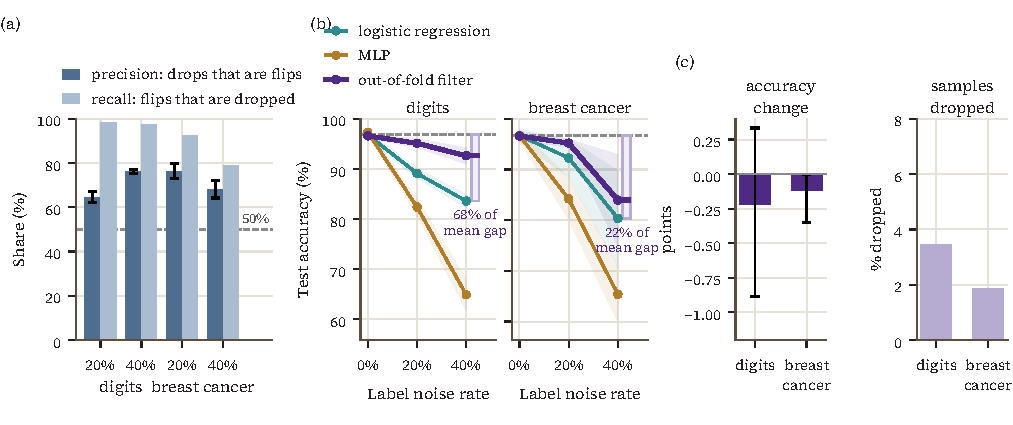
\includegraphics[width=0.96\textwidth]{figures/teaser.pdf}
\captionof{figure}{What the out-of-fold filter does, removes and gains. (a) A logistic regression fit on the other folds predicts each sample (1). It drops mismatches with the given label (2, 3) and refits once (4). Samples are schematic (fill marks the given class). (b) Share of the training set removed, split into mislabeled and correctly labeled; black side marks give the set's mislabeled share. (c) Test accuracy of ours minus that of logistic regression with the same settings (red zero line), paired by seed. Gray marks give the same difference for the clean-label reference, the accuracy lost to noise; no mean gain reaches them. Bars are 5\src{n_seeds}-seed means; in (c), error bars are sd and dots are seeds.}
\label{fig:teaser}

  \vspace{\dbltextfloatsep}
}]

\begin{abstract}
Label noise lowers the accuracy of linear classifiers.
We measure what a known remedy, an out-of-fold filter, removes, recovers and costs for logistic regression: it drops samples whose given labels disagree with a logistic regression fit on the other folds, then refits once, with no clean validation set, noise-rate estimate or confidence threshold.
On two small datasets, digits and breast cancer, at two symmetric noise rates, most drops are mislabeled, and the kept set is much cleaner than the training set.
In every noisy setting, the refit model's mean test accuracy exceeds that of logistic regression with the same settings (not significantly on breast cancer at the lower rate) but is below the clean-label reference, winning back only part of the lost accuracy.
With clean labels, few samples are removed, at little cost.

\end{abstract}

\section{Introduction}\label{sec:intro}

A logistic regression that has not seen a sample, and disagrees with its label, is usually right. On digits, dropping every such sample and refitting wins back most of the mean accuracy gap that label noise opens for logistic regression (the \emph{recovered share}: filter minus noisy logistic regression, divided by clean minus noisy logistic regression, from 5-seed means). On breast cancer the same rule recovers only 22\%\src{recovery_bc_n40} of the gap at 40\%\src{noise_max_pct} noise, and its gain at 20\%\src{noise_mid_pct} noise is not significant.

Labels collected at scale are often wrong, and a linear model trained on them pays for it: at 40\%\src{noise_max_pct} symmetric noise, logistic regression loses 13.2\src{loss_digits_n40} points of test accuracy on digits. Surveys list many repairs \citep{song2023learning,frenay2014classification}. Loss correction and reweighting need an estimate of the noise rate or a clean validation set \citep{patrini2017making,ren2018learning}, and practitioners often have neither. Our two datasets are small and nearly linearly separable, and symmetric flips are the most favorable case for a linear filter, so the results below say little about harder data.

We revisit a simpler idea, out-of-fold filtering of mislabeled data \citep{brodley1999identifying}, as a baseline that needs no side information. The out-of-fold filter fits logistic regression with cross-validation, drops every training sample whose out-of-fold prediction disagrees with its label, and refits on the rest. A flipped label contradicts the structure that the other labels share. Because the prediction is out-of-fold, the model has not seen the sample it judges, which should keep it from agreeing with a flipped label. The rule is not new. What we add is a measurement: its precision and recall against known flipped labels, the recovered share, and a comparison with a multilayer perceptron (MLP).

Figure~\ref{fig:teaser} shows what this buys. The disagreement is a precise and high-recall detector: on digits at 40\%\src{noise_max_pct} noise, 76\%\src{prec_digits_n40} of dropped samples are truly flipped and 98\%\src{rec_digits_n40} of flipped labels are dropped (Fig.~\ref{fig:teaser}a). Refitting on the kept samples recovers 68\%\src{recovery_digits_n40} of the mean gap there. A sanity check with an untuned MLP trained on the same noisy labels shows that the network degrades faster (Fig.~\ref{fig:teaser}b). On clean labels the filter costs little accuracy ($-$0.2\src{gain_digits_n0_vs_logreg} points on digits, $-$0.1\src{gain_bc_n0_vs_logreg} on breast cancer, neither significant), although it drops 3.5\%\src{dropped_frac_digits_n0} and 1.9\%\src{dropped_frac_bc_n0} of the clean samples (Fig.~\ref{fig:teaser}c). It does not reach clean-label accuracy at 40\%\src{noise_max_pct} noise.

\begin{figure*}[t]
  \centering
  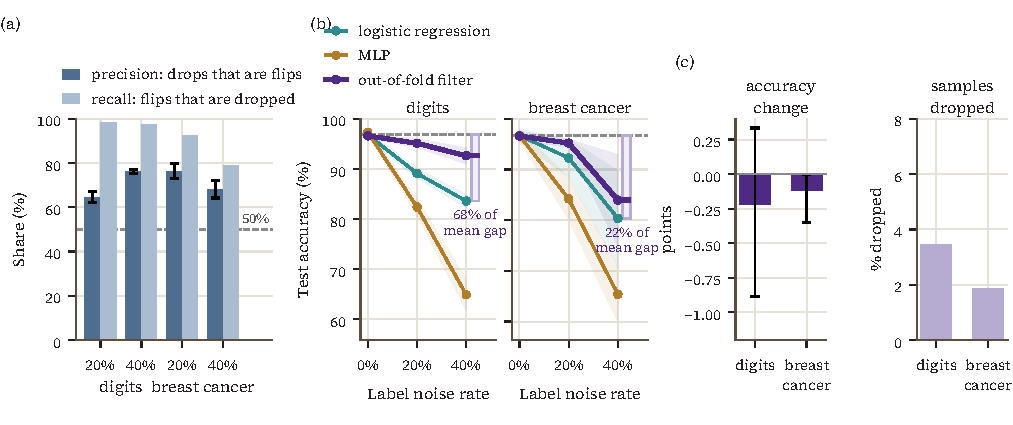
\includegraphics[width=\textwidth]{figures/teaser.pdf}
  \caption{Out-of-fold disagreement of logistic regression finds flipped labels, and dropping those samples wins back much of the mean accuracy gap that label noise opens on digits, but less on breast cancer. (a) Precision and recall of the drop set at two noise rates; the dashed line marks 50\%. (b) Test accuracy against noise for logistic regression, an untuned MLP and the out-of-fold filter; bands are sd over 5 seeds, and the box at the right edge marks the share of the mean gap won at 40\%\src{noise_max_pct} noise. (c) Cost of filtering on clean labels (no label flipped): paired accuracy change against logistic regression (95\% interval over 5 seeds) and share of clean samples dropped.}
  \label{fig:teaser}
\end{figure*}

We make three contributions.
\begin{itemize}
  \item We show that the out-of-fold disagreement of a logistic regression with a training label is a precise and high-recall detector of flipped labels on two datasets under symmetric noise.
  \item We evaluate the classical out-of-fold filter with one linear model and no side information, measuring the recovered share against noisy logistic regression.
  \item We show that it improves over logistic regression at 40\%\src{noise_max_pct} noise on both datasets and at 20\%\src{noise_mid_pct} on digits (not significant on breast cancer at 20\%\src{noise_mid_pct}), that it costs little on clean labels, and where it falls short. An untuned MLP serves as a sanity check.
\end{itemize}

\section{Related Work}\label{sec:related}

\paragraph{Learning with noisy labels.}
Surveys group methods for deep networks \citep{song2023learning} and for classical classifiers \citep{frenay2014classification} into a few families. Loss correction estimates a matrix of class-corruption probabilities and adjusts the loss \citep{patrini2017making}. Noise-tolerant losses are chosen so that the minimizer survives label noise \citep{ghosh2017robust}. Noise models can also sit inside logistic regression \citep{bootkrajang2014learning,lee2021individual}. The fourth family, sample selection, picks the training samples to trust. Our out-of-fold filter changes neither the loss nor the model and needs no noise model.

\paragraph{Sample selection in deep networks.}
In co-teaching, two networks exchange their small-loss samples \citep{han2018coteaching}. Co-teaching+ selects among the samples on which the two networks disagree \citep{yu2019how}. Area Under the Margin ranks samples by their training dynamics \citep{pleiss2020identifying}. These methods rely on deep-network training dynamics. We use the out-of-fold predictions of a linear model and do not compare against them.

\paragraph{Cross-validated filtering and confident learning.}
\citet{brodley1999identifying} filter a training set by removing the instances that classifiers misclassify, in single-algorithm, majority-vote and consensus variants. Confident learning prunes instances using out-of-sample predicted probabilities, per-class thresholds and an estimate of the number of label errors \citep{northcutt2021confident}. Our rule is the single-algorithm filter with logistic regression and a plain argmax disagreement. We add a checkable measurement of its precision, recall, accuracy gain and clean-label cost; we do not claim a new filtering idea. We do not compare against confident learning.

\section{Out-of-Fold Label Filtering}\label{sec:method}

\paragraph{Setting.}
The filter changes which samples logistic regression is fit on. The training set $D=\{(x_i,\tilde{y}_i)\}_{i=1}^{n}$ has $n$ samples, each a feature vector $x_i$ with a given label $\tilde{y}_i$ that may be wrong. The base model $f_D$ maps a feature vector to a class. It chains standardization and logistic regression, both fit on the set in its subscript. The logistic regression baseline is $f_D$, trained on all given labels without filtering.

\paragraph{Out-of-fold check.}
A model that has never seen a sample cannot have memorized a wrong label for it, so we check each given label with such a model. We shuffle $D$ and split it into $K$ cross-validation folds~\citep{stone1974crossvalidatory}, stratified on the given labels, and write $D_{k(i)}$ for the fold that contains sample $i$. We fit the base model, standardization included, on the other folds. The class it predicts for sample $i$ is the out-of-fold prediction $\hat{y}_i = f_{D \setminus D_{k(i)}}(x_i)$.

\paragraph{Keep rule and refit.}
We keep a sample only if its out-of-fold prediction equals its given label. The kept set is
\begin{equation}
  D_{\mathrm{keep}} = \{(x_i,\tilde{y}_i) \in D : \hat{y}_i = \tilde{y}_i\}.
  \label{eq:keep}
\end{equation}
We fit a new standardization and logistic regression on this set, which gives the refit model $f_{D_{\mathrm{keep}}}$ (Fig.~\ref{fig:teaser}a).

\paragraph{What the filter does not need.}
The filter needs no clean validation set or noise-rate estimate. It makes one pass over hard predictions, with no confidence threshold or per-class rule. The number of drops is the number of disagreements. We fix $K$ and the inverse regularization strength $C$ without tuning (Section~\ref{sec:setup}).

\section{Experimental setup}\label{sec:setup}

\paragraph{Data and noise.}
We use 2\src{n_datasets} scikit-learn datasets: digits (ten classes) and breast cancer (two classes). Each is split with stratification into a training set and a test set holding 30\%\src{test_fraction_pct} of the samples, with a new split per seed. Digits has 1,257\src{n_train_digits} training and 540\src{n_test_digits} test samples, and breast cancer has 398\src{n_train_bc} and 171\src{n_test_bc}. Symmetric noise flips each training label with probability 0, 20\%\src{noise_mid_pct} or 40\%\src{noise_max_pct} to a uniformly drawn other class. The sampled flip rate at nominal 40\%\src{noise_max_pct} is slightly lower: 39.4\%\src{actual_noise_digits_n40} on digits and 38.6\%\src{actual_noise_bc_n40} on breast cancer. Test labels stay clean.

\paragraph{Methods.}
We compare three methods. The out-of-fold filter uses $K=$5\src{filter_folds} folds. Logistic regression ($C=$1\src{logreg_c}) trains on the noisy labels and doubles as the no-filter ablation. The multilayer perceptron (MLP) has one hidden layer of 64\src{mlp_hidden} units, scikit-learn defaults, and up to 500\src{mlp_max_iter} iterations; it is untuned, unregularized and has no early stopping. No oracle run exists, so logistic regression on clean labels serves as the reference for the recovered share. We tuned neither $C$ nor $K$, and we ran no other cheap baseline (a smaller or cross-validated $C$, co-teaching, confident learning, small-loss filtering, or the same filter with another learner). The gain of the filter over logistic regression at $C=1$ may therefore partly reflect regularization strength and training-set size: at 40\%\src{noise_max_pct} noise the filter refits on about half of the data, 623\src{kept_digits_n40} of 1,257\src{n_train_digits} samples on digits and 221\src{kept_bc_n40} of 398\src{n_train_bc} on breast cancer.

\paragraph{Metrics and statistics.}
Test accuracy uses the clean test labels. Precision is the share of dropped samples that were flipped, and recall is the share of flipped labels that were dropped. The recovered share is (filter minus noisy logistic regression) divided by (clean minus noisy logistic regression), computed from 5-seed means and carrying no interval; the clean-label reference is not an oracle. Each cell uses 5\src{n_seeds} seeds, a small fixed budget, paired across methods by a shared split and noise draw, for 90\src{n_runs_total} runs in total. We report paired t-tests and confidence intervals of paired differences, obtained by resampling the five paired differences; tables give mean $\pm$ sd. The tests are uncorrected, the paired seeds share splits, and the $p$-values assume approximately normal differences. With 5 seeds an interval can exclude zero while the $t$-test does not, so we call such gains suggestive.

\subsection{Under noise, the kept set is much cleaner}\label{sec:results_drops}

\begin{table*}[t]
\centering
\small
\caption{What the out-of-fold filter drops at 20\% and 40\% label noise. Precision is the share of dropped samples that were flipped, recall the share of flipped samples that were dropped, and $p$ tests precision against 50\% (two-sided one-sample $t$-test). Recovered is the share of logistic regression's accuracy loss that the filter regains (our definition). Means over 5\src{n_seeds} seeds; clean-label rows are omitted because precision and recall are undefined there. The filter removes mostly flipped samples in every setting.}
\label{tab:drops}
\begin{tabular}{lccccc}
\toprule
Setting & Dropped & Precision (\%) & $p$ vs 50\% & Recall (\%) & Recovered (\%) \\
\midrule
Digits, 20\% & 377.4\src{dropped_digits_n20} & 64.6\src{precision_digits_n20} & $1.5\times 10^{-4}$\src{p_prec_dg20_gt50} & 98.5\src{recall_digits_n20} & 77.9\src{recovered_digits_n20} \\
Digits, 40\% & 634.2\src{dropped_digits_n40} & 76.1\src{precision_digits_n40} & $2.1\times 10^{-7}$\src{p_prec_dg40_gt50} & 97.5\src{recall_digits_n40} & 68.3\src{recovered_digits_n40} \\
Breast cancer, 20\% & 92.8\src{dropped_breast_cancer_n20} & 76.4\src{precision_breast_cancer_n20} & $6.5\times 10^{-5}$\src{p_prec_bc20_gt50} & 92.5\src{recall_breast_cancer_n20} & 65.8\src{recovered_breast_cancer_n20} \\
Breast cancer, 40\% & 177.2\src{dropped_breast_cancer_n40} & 68.3\src{precision_breast_cancer_n40} & $5.5\times 10^{-4}$\src{p_prec_bc40_gt50} & 78.9\src{recall_breast_cancer_n40} & 22.1\src{recovered_breast_cancer_n40} \\
\bottomrule
\end{tabular}
\end{table*}


\paragraph{Removal grows with noise and exceeds the flipped share.}
The filter is never told the noise rate, yet it removes more samples as that rate grows. In every noisy setting, it removes a larger share of the training set than was flipped (Table~\ref{tab:drops}, Fig.~\ref{fig:teaser}b). With clean labels, where every drop is correctly labeled, it removes only 3.5\%\src{drop_fraction_digits_noise0} of the training set on digits and 1.9\%\src{drop_fraction_breast_noise0} on breast cancer.

\paragraph{The filter selects far better than chance.}
Removing as many samples at random would, in expectation, leave the mislabeled share unchanged, with drop precision equal to the flipped share and drop recall equal to the share of the training set removed. In every noisy setting, the filter does much better: its kept set has a far smaller mislabeled share than the training set, and its drop precision and recall are well above those chance levels (Table~\ref{tab:drops}). Most drops are mislabeled in every noisy run, but a sizable minority are correctly labeled, with drop precision ranging from 61\%\src{drop_precision_min} to 81\%\src{drop_precision_max} across these runs. The kept set has by far the largest mislabeled share on breast cancer at the higher rate.

\paragraph{Heavier noise worsens both kinds of error.}
On seed means, the filter at the higher rate misses more of the flipped labels and also discards a larger share of the correctly labeled samples on both datasets (Table~\ref{tab:drops}). Its drop precision stays above the flipped share, but by a smaller factor than at the lower rate.

\subsection{Refitting wins back part of the lost accuracy}\label{sec:results_accuracy}

\begin{table*}[t]
\centering
\small
\caption{Test accuracy (\%) on clean test labels by dataset and symmetric training-label noise rate. Mean $\pm$ sd over 5\src{n_seeds} seeds, each a re-drawn stratified split with 540\src{n_test_digits} test samples on digits and 171\src{n_test_breast} on breast cancer. Logistic regression with clean labels is the clean-label reference. Bold marks the best column mean, ties included. Ours has the highest mean in each noisy setting, but not with clean labels.}
\label{tab:accuracy}
\begin{tabular}{lcccccc}
\toprule
& \multicolumn{3}{c}{Digits} & \multicolumn{3}{c}{Breast cancer} \\ \cmidrule(lr){2-4} \cmidrule(lr){5-7} Method & Clean & 20\%\src{noise_rate_low} & 40\%\src{noise_rate_high} & Clean & 20\%\src{noise_rate_low} & 40\%\src{noise_rate_high} \\
\midrule
Logistic regression & 96.8\src{acc_logreg_digits_noise0} $\pm$ 0.8\src{std_logreg_digits_noise0} & 89.1\src{acc_logreg_digits_noise20} $\pm$ 1.0\src{std_logreg_digits_noise20} & 83.6\src{acc_logreg_digits_noise40} $\pm$ 1.3\src{std_logreg_digits_noise40} & \textbf{96.7}\src{acc_logreg_breast_noise0} $\pm$ 1.2\src{std_logreg_breast_noise0} & 92.3\src{acc_logreg_breast_noise20} $\pm$ 3.7\src{std_logreg_breast_noise20} & 80.4\src{acc_logreg_breast_noise40} $\pm$ 9.4\src{std_logreg_breast_noise40} \\
MLP & \textbf{97.3}\src{acc_mlp_digits_noise0} $\pm$ 0.5\src{std_mlp_digits_noise0} & 82.4\src{acc_mlp_digits_noise20} $\pm$ 1.6\src{std_mlp_digits_noise20} & 64.9\src{acc_mlp_digits_noise40} $\pm$ 3.1\src{std_mlp_digits_noise40} & \textbf{96.7}\src{acc_mlp_breast_noise0} $\pm$ 1.2\src{std_mlp_breast_noise0} & 84.2\src{acc_mlp_breast_noise20} $\pm$ 4.0\src{std_mlp_breast_noise20} & 65.4\src{acc_mlp_breast_noise40} $\pm$ 5.4\src{std_mlp_breast_noise40} \\
Filter (ours) & 96.6\src{acc_filter_digits_noise0} $\pm$ 0.4\src{std_filter_digits_noise0} & \textbf{95.1}\src{acc_filter_digits_noise20} $\pm$ 0.9\src{std_filter_digits_noise20} & \textbf{92.6}\src{acc_filter_digits_noise40} $\pm$ 1.6\src{std_filter_digits_noise40} & 96.6\src{acc_filter_breast_noise0} $\pm$ 1.0\src{std_filter_breast_noise0} & \textbf{95.2}\src{acc_filter_breast_noise20} $\pm$ 0.8\src{std_filter_breast_noise20} & \textbf{84.0}\src{acc_filter_breast_noise40} $\pm$ 9.0\src{std_filter_breast_noise40} \\
\bottomrule
\end{tabular}
\end{table*}


\paragraph{Filtering mostly beats training on all noisy labels.}
Ours has a higher mean test accuracy than logistic regression with the same settings in every noisy setting and is ahead in all noisy runs but one (Table~\ref{tab:accuracy}, Fig.~\ref{fig:teaser}c). The difference is established on digits at both rates and on breast cancer at the higher rate, but not on breast cancer at the lower rate ($p = 0.12$\src{p_filter_vs_logreg_breast_noise20}). We ran no random-drop or oracle control, so we do not attribute the gain to removing the right samples.

\paragraph{The clean-label reference is not reached.}
The filter's mean test accuracy stays below the clean-label reference in all four noisy settings (gray marks in Fig.~\ref{fig:teaser}c). Both gaps at the lower rate are borderline: the gap on digits just misses the five percent level ($p = 0.053$\src{p_clean_logreg_vs_filter_digits_noise20}), and the gap on breast cancer just passes it ($p = 0.049$\src{p_clean_logreg_vs_filter_breast_noise20}). Both gaps at the higher rate also pass it. Because the test likely overstates significance, we read all four gap verdicts as tentative.

\paragraph{The share of lost accuracy won back differs by setting.}
On seed means, the filter wins back much of the lost accuracy on digits at both rates (Table~\ref{tab:drops}). The same holds on breast cancer at the lower rate. There, however, the gain over logistic regression is not established, and the share of lost accuracy won back is unstable, ranging from $-67$\%\src{recovered_seed_min_breast_noise20} to 100\%\src{recovered_seed_max_breast_noise20} across seeds.

\paragraph{Breast cancer at the higher rate is the weak case.}
The filter wins back only a small part of the loss there. The two seeds where ours and logistic regression are least accurate have the most flipped labels (41.7\src{flipped_low_seeds_min_breast_noise40} to 42.2\%\src{flipped_low_seeds_max_breast_noise40}, others 35.4\src{flipped_other_seeds_min_breast_noise40} to 37.9\%\src{flipped_other_seeds_max_breast_noise40}) and the largest mislabeled shares of the kept set (at least 18\%\src{kept_noisy_low_seeds_min_breast_noise40}, others at most 13\%\src{kept_noisy_other_seeds_max_breast_noise40}). This is an association over five seeds; our runs do not show what causes it.

\paragraph{A larger model does not make filtering unnecessary here.}
The MLP trained on all noisy labels is less accurate than ours in every noisy run (Table~\ref{tab:accuracy}). Logistic regression also beats it in every noisy run, so this gap says nothing about what filtering adds or about larger models in general.

\subsection{On clean labels, the filter costs little}\label{sec:results_clean}

Discarding correctly labeled samples costs little accuracy when the labels are already clean (Table~\ref{tab:accuracy}, Fig.~\ref{fig:teaser}c). On digits, the test accuracy of ours minus that of logistic regression ranges from $-1.3$\src{gain_seed_min_digits_noise0} to $+0.6$\src{gain_seed_max_digits_noise0} percentage points across seeds. On breast cancer, the test accuracies of the two models differ in one seed only, by one test sample. Neither mean difference is established, but this does not show that the models are equivalent.

\section{Discussion and Limitations}\label{sec:discussion}

Checking each label against a model that never saw it is a simple way to clean a small training set for a linear classifier. In the tested settings, one fixed filter runs without being told the noise rate, or whether the labels are noisy at all, and under noise it leaves a much cleaner training set. It does not restore clean-label accuracy: its mean test accuracy stays below the clean-label reference in all four noisy settings. It also discards correctly labeled samples, and on breast cancer at the higher rate, many mislabeled ones survive it.

\paragraph{Limitations and next steps.}
We studied two small datasets, synthetic symmetric noise at two rates, one filtering pass with fixed $K$ and $C$, and one untuned MLP, which we did not combine with the filter. We tested the filter only where the clean-label reference is very accurate. Removing samples at a fixed $C$ also changes the relative strength of regularization, and we did not try stronger regularization without filtering. Without random-drop, oracle or in-sample filter controls, we cannot separate the effects of surviving mislabeled samples, lost correctly labeled samples and a smaller training set. We ran neither co-teaching~\citep{han2018coteaching} nor confident learning~\citep{northcutt2021confident} and claim no advantage over either. Next steps are these missing runs, class-dependent noise, other rates, and softer or repeated filtering.


{\small
\bibliographystyle{ieeenat_fullname}
\bibliography{refs}
}

\end{document}
